\documentclass{article}

\usepackage[margin=3cm]{geometry}

\usepackage{tikz-bagua}
\usetikzlibrary{math}
\usepackage{ctex}%[fontset=kefonts]

\input{binhex}

\usepackage{makeidx}   %创建索引

\makeindex  

\title{TikZ-Bagua 宏包}
\author{WANG Xu \\ cwangx@hotmail.com}
\date{\zhtoday~v1.01}

\begin{document}

\maketitle

\section{简介}

\verb+TikZ-Bagua+ 宏包使用 \verb+TikZ+ 宏包, 借助于 \verb+xparse+, \verb+xstring+, \verb+bitset+ 以及 \verb+xintexpr+, 定义了 \verb+\taiji+, \verb+\liangyi+, \verb+\sixiang+, 三爻 \verb+\bagua+ 和六爻 \verb+\Bagua+,  画出《周易》中所用的的太极阴阳, 两仪四象八卦和六十四卦符号, 对字体没有要求.

\section{使用方法}

所定义的上述五个命令中最后一个可选参数均为放缩参数 \verb|scale|, 缺省值均为 $1$.

\subsection{太极阴阳}

感谢热心网友的指出, 默认是古籍中的太极图, 且没有鱼眼, 加星则显示鱼眼. 鉴于现在常见到的半圆构造的也不少, 故新增命令以显示之, 显示鱼眼规则同上. 

\verb+\taiji [<scale>]+\index{taiji@\verb+\taiji+}, \verb+\taiji* [<scale>]+\index{xtaiji@\verb+\xtaiji+}.

\verb+\xtaiji [<scale>]+\index{taiji@\verb+\taiji+}, \verb+\xtaiji* [<scale>]+\index{xtaiji@\verb+\xtaiji+}.

四个命令默认直接对应得到 符号 \taiji \taiji* \xtaiji \xtaiji*.

\subsection{两仪}
\verb+\liangyi {<bin>} [<scale>]+\index{liangyi@\verb+\liangyi+}.

\verb+\liangyi{<bin>}+ 通过接受参数 $1$ 或 $0$ 得到两仪符号 \liangyi{1} 或 \liangyi{0}.

\subsection{四象}
\verb+\sixiang {<bin>} [<scale>]+\index{sixiang@\verb+\sixiang+}, \verb+\sixiang* {<dec>} [<scale>]+\index{sixiang*@\verb+\sixiang*+}.

\verb+\sixiang{<bin>}+ 通过接受参数 $3,2,1,0$ 的二进制数得到四象符号, 而 \verb+\sixiang*{<dec>}+ 接收十进制数.

\begin{center}
	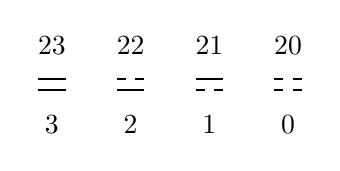
\begin{tikzpicture}
		\foreach \j in {3,2,1,0}
		{
			\node at (3-\j,-0.5) {$\j$};
			\node at (3-\j,0.5) {\nbinary{2}{\j}};
			\node at (3-\j,0) {\sixiang*{\j}};
		}
	\end{tikzpicture}
\end{center}

\subsection{三爻八卦}
\verb+\bagua {<bin>} [<scale>]+\index{bagua@\verb+\bagua+}, \verb+\bagua* {<dec>} [<scale>]+\index{bagua*@\verb+\bagua*+}.

\verb+\bagua{<bin>}+ 通过接受参数 $7,6,\dots,0$ 的二进制数得到三爻八卦符号, 而 \verb+\bagua*{<dec>}+ 接收十进制数.

\begin{center}
	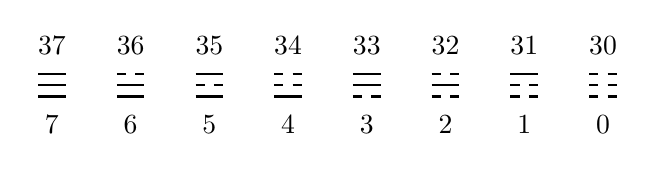
\begin{tikzpicture}
		\foreach \j in {7,6,...,0}
		{
			\node at (7-\j,-0.5) {$\j$};
			\node at (7-\j,0.5) {\nbinary{3}{\j}};
			\node at (7-\j,0) {\bagua*{\j}};
		}
	\end{tikzpicture}
\end{center}

\subsection{六爻八卦}
\verb+\Bagua [<2,8>]{<bin,oct>} [<scale>]+\index{Bagua@\verb+\Bagua+}, \verb+\Bagua* {<dec>} [<scale>]+\index{Bagua*@\verb+\Bagua*+}.

\verb+\Bagua{<bin>}+ 通过接受参数 $63,62,\dots,0$ 的二进制数得到六爻八卦符号, \verb+\Bagua[8]{<oct>}+ 接收的为$63,62,\dots,0$ 的八进制数, 而 \verb+\Bagua*{<dec>}+ 接收十进制数.

列出所有的六十四卦, 其中每卦上一行六位数为对应的二进制数, 下一行左右两边分别为对应的十进制和八进制数.

\begin{center}
	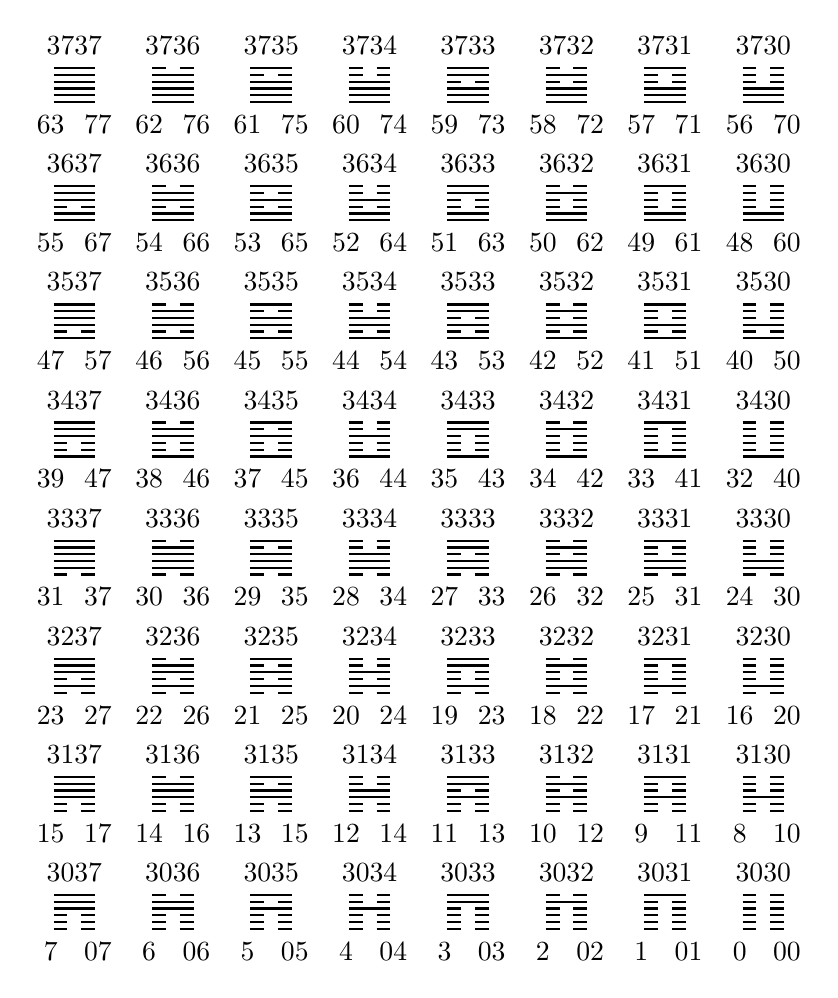
\begin{tikzpicture}
		\foreach \j in {7,6,...,0}
		{
			\foreach \k in {7,6,...,0}
			{
				\node at (7*1.25-1.25*\k-0.3,1.5*\j-0.5) {\pgfmathparse{int(8*\j+\k)}\pgfmathresult};
				\node at (7*1.25-1.25*\k+0.3,1.5*\j-0.5) {\j\k};
				\node at (7*1.25-1.25*\k,1.5*\j+0.5) {\nbinary{3}{\j}\nbinary{3}{\k}};
				\node at (7*1.25-1.25*\k,1.5*\j) {\Bagua[8]{\j\k}[1.5]};
			}
%			\node at (7-\j,0) {$\j$};
%			\node at (7-\j,-0.5) {\nbinary{3}{\j}};
%			\node at (7-\j,-1) {\bagua*{\j}};
		}
	\end{tikzpicture}
\end{center}

\section{版本记录}
\subsection*{v1.01~2022.08.04}
修改默认 \verb+\taiji+ 为无鱼眼的古籍上的太极, 为现在常见的半圆构造新增 \verb+\xtaiji+, 修复了已发现的 bug.

\subsection*{v1.0~2021.10.17}
发布 \verb+TikZ-Bugua+ 宏包.

\printindex

\end{document}